\subsection{Revisiting Pass@K Experiments for Skywork-OR1}
\label{supp_sec:benchmark_skywork_or1}

Skywork-OR1~\citep{he2025Skywork-OR1} has generously shared their complete training recipes, claiming to enhance distilled LLMs with more powerful reasoning capabilities through RLVR. Therefore, we conduct the Pass@K experiments on their models to understand how RLVR could improve distilled LLMs.

Figure~\ref{fig:cot_passk_code_bench_skywork} shows the Pass@K comparisons between Skywork-OR1-7B and DeepSeek-R1-Distill-Qwen-7B on LiveCodeBench-v6. We can also observe a significant improvement of both sampling efficiency (Pass@1) and reasoning boundary (Pass@K, K up to 1024). This conclusion is consistent with the observations for Figure~\ref{fig:cot_passk_code_bench_ace} in the main paper.

\begin{figure}[ht]
\begin{center}
%\framebox[4.0in]{$\;$}
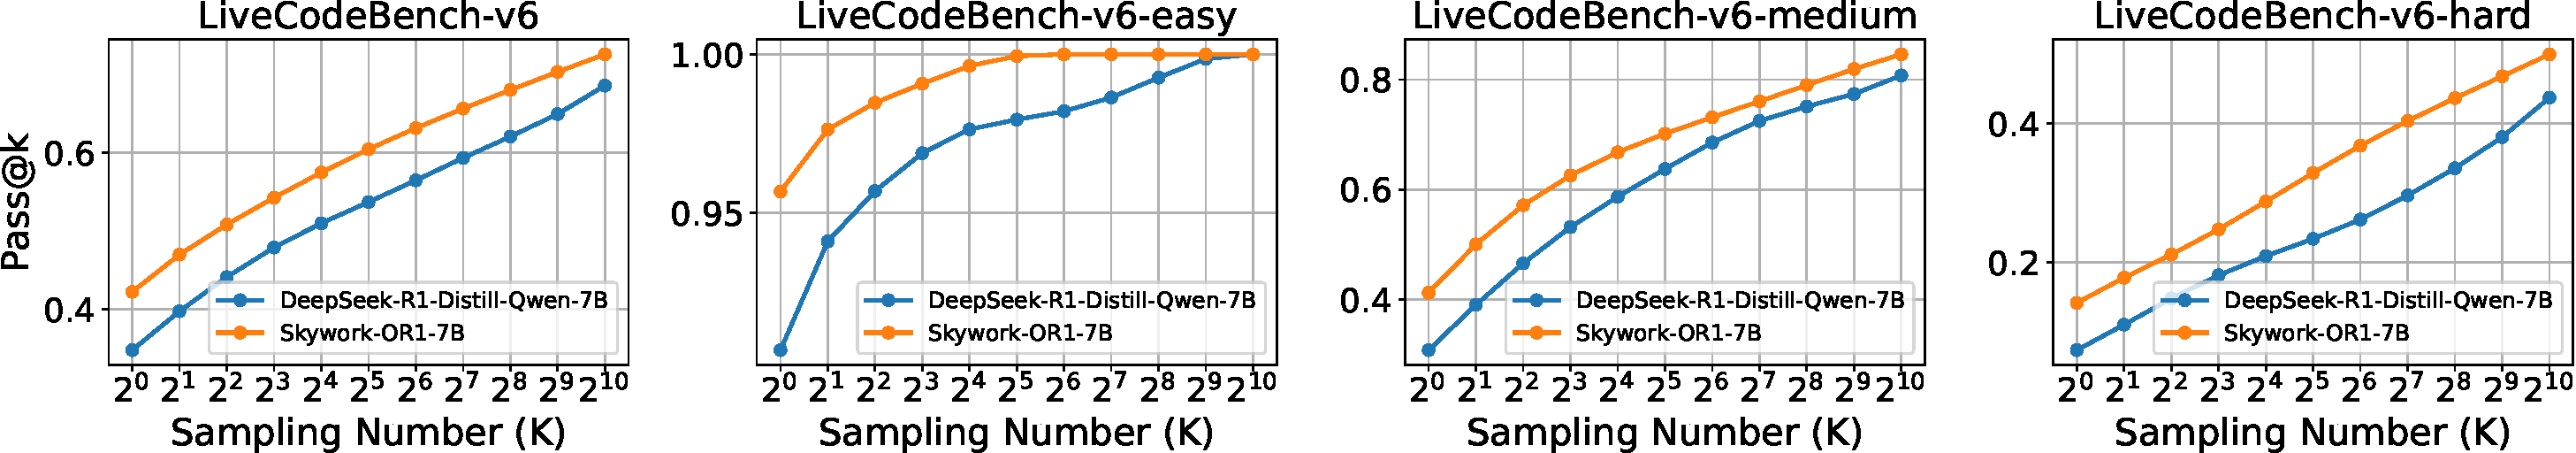
\includegraphics[width=1.0\textwidth]{figures/wxm_eval_skywork_lcb_v6.pdf}
\end{center}
\caption{Comparisons of Pass@K on LiveCodeBench-v6 and its different difficulty-level subsets. Here the distilled LLM is DeepSeek-R1-Distill-Qwen-7B, and the post-RLVR model is Skywork-OR1-7B.}
\label{fig:cot_passk_code_bench_skywork}
\end{figure}

However, in math domains, applying RLVR to distilled LLMs seems to merely deliver sampling efficiency improvements.
As shown in Figure~\ref{fig:cot_passk_math_bench_skywork}, we observe that even using the CoT-Pass@K metric, Skywork-OR1-Math-7B and DeepSeek-R1-Distill-Qwen-7B do not have distinct Pass@K gaps for large K values.
We suspect the reason is that the distilled LLM may already master major reasoning capabilities that can be learned with RLVR using answer correctness as the reward.
So in math domains, their main improvements lie in Pass@1.
In contrast, for code domains, applying RLVR to distilled LLMs can still stimulate them to fit for real-world execution feedback, thereby incentivizing extended reasoning boundary.

\begin{figure}[h]
\begin{center}
%\framebox[4.0in]{$\;$}
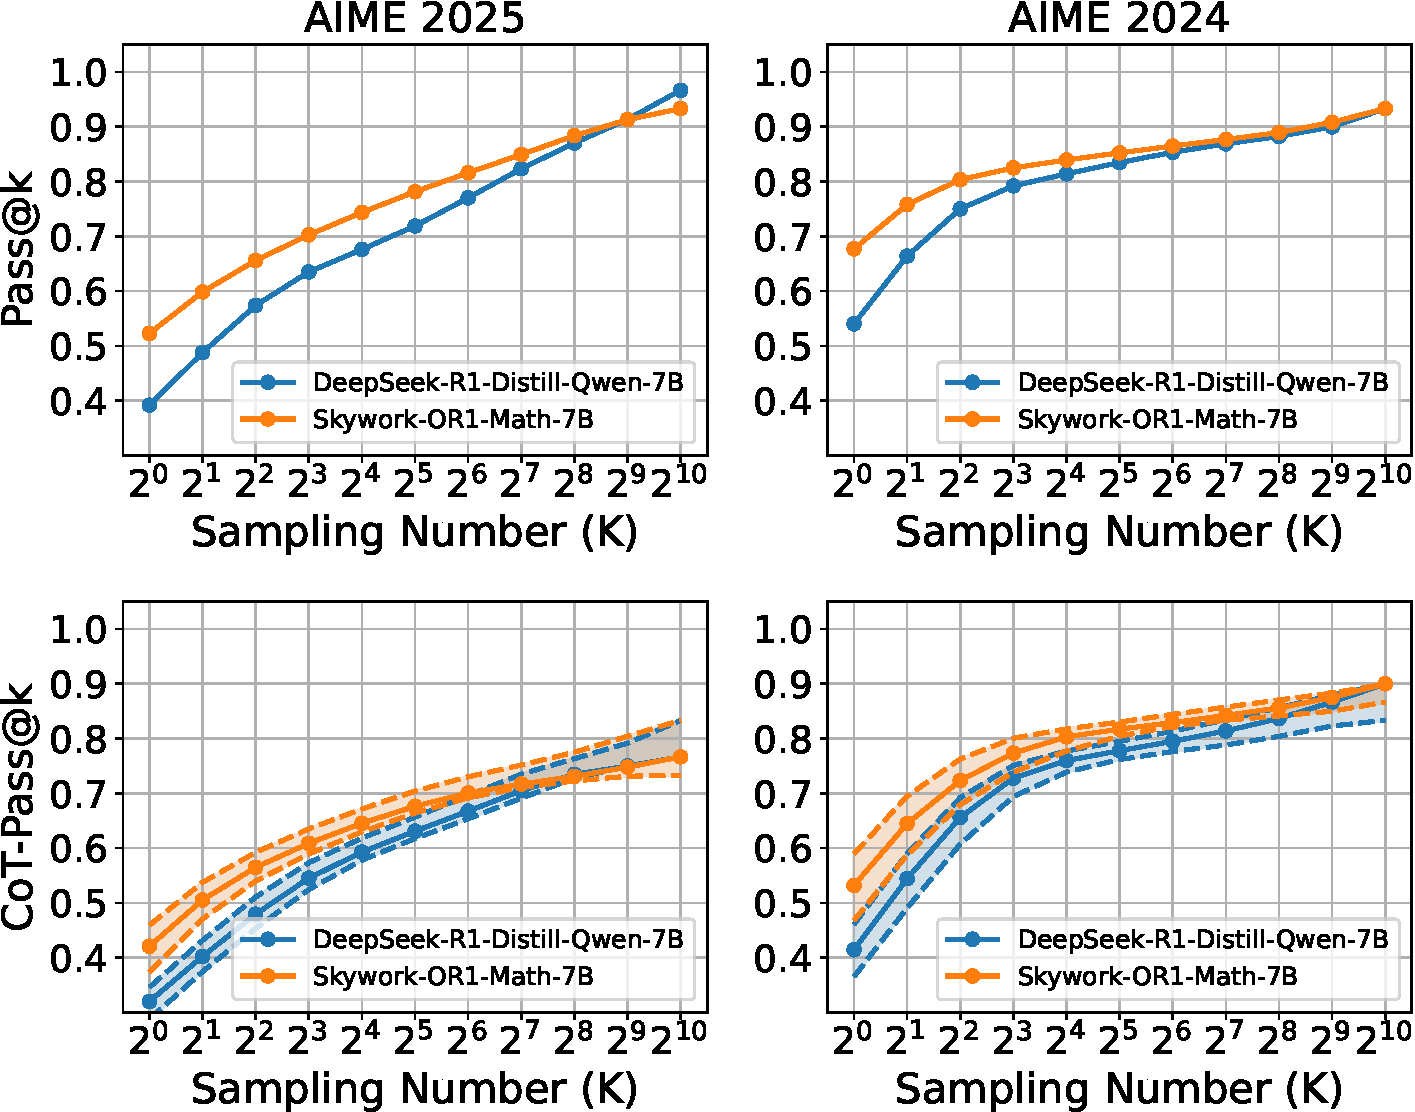
\includegraphics[width=0.65\textwidth]{figures/wxm_eval_skywork_aime.pdf}
\end{center}
\caption{Comparisons of Pass@K (the top row) and CoT-Pass@K (the bottom row) on AIME 2024, 2025 to show how RLVR could improve distilled LLMs. Here the distilled LLM is DeepSeek-R1-Distill-Qwen-7B, and the post-RLVR model is Skywork-OR1-Math-7B. For CoT-Pass@K, we perform multiple verifications for each CoT using DeepSeek-R1-0528-Qwen3-8B, and display the results determined by \emph{any-correct}, \emph{all-correct}, and \emph{majority-correct} strategies, which constitute the shaded area in lower subplots.}
\label{fig:cot_passk_math_bench_skywork}
\end{figure}
